%=====================================================================
\part{The evolution of the network}\label{part:evolution}
%=====================================================================
\chapter{Evolution of the effect and resource networks}\label{ch:evoE}

Part I treated the two quantum networks (GPT, QRT) as finished objects with a version axis, and the readers and the Standard Model history as graphs with a native time index (paragraph, step). This part puts all four on one calendar axis and derives how each grew, node by node and edge by edge. The quantum networks have no time axis of their own; what they have is a reference list on every edge, and on every node of the resource-theory network. The chronology below is computed from those references by rules stated once, and every number in this part is the output of \texttt{build\_evolution.py} on the same released data as Part I.

\section{A calendar axis from the references}\label{sec:dating}
\begin{definition}[year index of a type-E graph]\label{def:dating}
Let $G=(V,R)$ be an effect or resource network whose routes $r$ carry reference strings $\mathrm{refs}(r)$ and whose nodes may carry $\mathrm{refs}(v)$. For a reference string, its \emph{year} is the publication year in parentheses, or the year encoded in an arXiv identifier; a bare four-digit number placed like a page number is not a year. Then
\begin{itemize}[nosep]
\item $t(r)=\min\{\text{year of } s : s\in\mathrm{refs}(r)\}$: the earliest cited source (provenance \emph{cited});
\item $t(v)=\min\bigl(\{\text{year of } s: s\in\mathrm{refs}(v)\}\cup\{t(r): v\in r,\ t(r)\text{ defined}\}\bigr)$ (provenance \emph{node-ref} or \emph{edge});
\item $t(r)=\max\{t(u): u\in r\}$ if $r$ cites nothing dated (provenance \emph{propagated});
\item $t(v)=2026$ if no incident route and no node reference is dated (provenance \emph{project}).
\end{itemize}
A route whose references include a textbook or review phrase (``standard'', ``see'', ``review'') is flagged \emph{review-dated}. For the readers, $t$ of a paragraph is the first year mentioned in its text, carried forward within a section (fallback: the section's first year); a node is dated by its first paragraph and a route by $\max$ of its paragraph's year and its endpoints' years. For the Standard Model history, a node is dated by the first year of its \texttt{years} field (fallback: the start year of the first step that draws it) and a route by $\max$ of its step's start year and its endpoints' years.
\end{definition}

\begin{lemma}[the year index is a filtration]\label{lem:filtration}
Under \cref{def:dating}, $t(u)\le t(r)$ for every route $r$ and every endpoint $u\in r$ in all four branches.
\end{lemma}
\begin{proof}
For a type-E graph: a node dated by an incident route takes the minimum over its incident dated routes, hence $t(v)\le t(r)$ for every dated $r\ni v$; a node dated by its own reference is only earlier; a propagated route takes the maximum of its endpoints; a project-dated node has no dated incident route, so every route through it is propagated and dated $2026=t(v)$. For the readers and the history the route year is defined as a maximum that includes its endpoints. The engine asserts the inequality after dating; the count of violations is \EGPTForward{} (GPT) and \EQRTForward{} (QRT); for EM, \EemAdjusted{} of \EEMEfin{} routes and for HEP \EhepAdjusted{} of \EhepUnionRoutes{} routes had to be moved later than their paragraph or step year to satisfy it, which is the \emph{adjusted} provenance.
\end{proof}

\begin{table}[htbp]\centering\small
\caption{Provenance of the year index. Node years: \emph{edge} = earliest incident dated route; \emph{node-ref} = the node's own references (QRT); \emph{project} = no dated source, set to 2026; \emph{paragraph}/\emph{carried}/\emph{section} = the reader's text; \emph{node-years}/\emph{step} = the history's fields. Route years: \emph{cited}/\emph{review-dated}/\emph{propagated}; \emph{step+endpoints}, \emph{endpoints} = $\max$ rule.}\label{tab:evo_prov}
\begin{tabular}{@{}lp{5.6cm}p{6.2cm}@{}}\toprule
Branch & Node years (provenance: count) & Route years (provenance: count) \\\midrule
EM & carried 17, paragraph 102, section 1 & carried 13, paragraph 88, propagated 20, section 1 \\
HEP & node-years 76, step 2 & endpoints 24, step+endpoints 190 \\
GPT & edge 89, project 3 & cited 148, propagated 4, review-dated 4 \\
QRT & edge 19, node-ref 92, project 5 & cited 77, propagated 9 \\
\bottomrule\end{tabular}

\end{table}

\Cref{tab:evo_prov} gives the provenance counts. In the nonclassicality network \EGPTProvroutecited{} of \EGPTEfin{} routes are dated by a cited source and \EGPTProvnodeedge{} of \EGPTVfin{} nodes by an incident route; \EgptProjectNodes{} nodes carry no dated source (the unitary-dynamics, sharp-measurement and incompatible-set process nodes) and are placed at 2026. In the resource-theory network \EqrtNodeRef{} of \EQRTVfin{} nodes are dated by their own references and \EqrtProjectNodes{} are project-dated.

\section{What the years mean}\label{sec:dating-caveat}
The year index is an \emph{ingredient chronology}: a route is placed at the year of the oldest work it cites, which is the year from which its ingredients were available in print, not the year the route was established. The data cite sources selectively, so the ingredient year can precede the historical origin of a concept or follow it:
\begin{itemize}[nosep]
\item Bell nonlocality (\id{e-bell}) and its witness are dated 1969 because the route cites Clauser--Horne--Shimony--Holt \citep{chsh1969} and not Bell's 1964 paper \citep{bell1964}; Kochen--Specker contextuality (\id{e-ks}) is dated 1990 by Mermin \citep{mermin1990} rather than 1967 \citep{kochen1967}; entangled states (\id{s-ent}) are dated 1989 by Werner \citep{werner1989} rather than 1935 \citep{epr1935,schrodinger1935}; Wigner negativity (\id{s-wneg}) is dated 1946 by Groenewold \citep{groenewold1946} rather than 1932 \citep{wigner1932}, with Hudson's theorem \citep{hudson1974} among the later citations.
\item Conversely a route proved recently can be dated early by a background citation: the composed corollary \id{R3} (entangled states $\to$ generalised contextuality) cites Plávala--Gühne 2024 together with Werner 1989 and is dated 1989.
\end{itemize}
The ordering is therefore the ordering of the sources the networks' authors chose, and the thesis makes no historical claim beyond that. Two checks bound the effect of the convention. First, project-dated members are excluded from every lag statistic below and marked in the tables. Second, the whole analysis is recomputed with the \emph{latest} cited source as the route year (an upper bound on the establishment year) in \cref{tab:evo_robust}: node years move by \EGPTMaxShiftMean{} years on average in GPT (\EGPTMaxShiftZero{} of \EGPTVfin{} nodes unchanged) and by \EQRTMaxShiftMean{} years in QRT (\EQRTMaxShiftZero{} of \EQRTVfin{} unchanged); the closure fraction, the densification exponent and the preferential-closure ratio of \cref{ch:growth} change little (GPT: \EGPTClosureFrac\% $\to$ \EGPTMaxClosureFrac\%, $\alpha$ \EGPTAlpha{} $\to$ \EGPTMaxAlpha{}, ratio \EGPTPAratio{} $\to$ \EGPTMaxPAratio{}; QRT: \EQRTClosureFrac\% $\to$ \EQRTMaxClosureFrac\%, $\alpha$ \EQRTAlpha{} $\to$ \EQRTMaxAlpha{}, ratio \EQRTPAratio{} $\to$ \EQRTMaxPAratio{}), while the latencies shrink (GPT median \EGPTLatMedian{} $\to$ \EGPTMaxLatMedian{} years). The conclusions drawn below are the ones that survive this change.

\begin{table}[htbp]\centering\small
\caption{Robustness of the growth quantities of the effect networks to the dating convention: earliest cited source (the convention of this thesis) against latest cited source. Latency: median years between the later endpoint and the closure route. $\alpha$: densification exponent (\cref{sec:densification}). PA: preferential-closure ratio (\cref{sec:pa}).}\label{tab:evo_robust}
\begin{tabular}{@{}llrrrrrr@{}}\toprule
Branch & convention & first year & closure frac. & latency median & $\bar d_{\mathrm{arr}}$ & $\alpha$ & PA \\\midrule
GPT & earliest & \EGPTYZero{} & \EGPTClosureFrac\% & \EGPTLatMedian{} & \EGPTMeanArrDeg{} & \EGPTAlpha{} & \EGPTPAratio{} \\
GPT & latest & \EGPTMaxYZero{} & \EGPTMaxClosureFrac\% & \EGPTMaxLatMedian{} & \EGPTMaxMeanArrDeg{} & \EGPTMaxAlpha{} & \EGPTMaxPAratio{} \\
QRT & earliest & \EQRTYZero{} & \EQRTClosureFrac\% & \EQRTLatMedian{} & \EQRTMeanArrDeg{} & \EQRTAlpha{} & \EQRTPAratio{} \\
QRT & latest & \EQRTMaxYZero{} & \EQRTMaxClosureFrac\% & \EQRTMaxLatMedian{} & \EQRTMaxMeanArrDeg{} & \EQRTMaxAlpha{} & \EQRTMaxPAratio{} \\
\bottomrule\end{tabular}
\end{table}

\section{Arrivals and closures}\label{sec:arrivals}
\begin{definition}[arrival and closure]\label{def:arrival}
In a dated graph, a route $r$ is an \emph{arrival route} if at least one endpoint has $t(u)=t(r)$ (it is dated the year one of its nodes appears) and a \emph{closure route} if every endpoint satisfies $t(u)<t(r)$. The \emph{degree at arrival} of a node $v$ is $d_{\mathrm{arr}}(v)=|\{r\ni v: t(r)=t(v)\}|$. The \emph{latency} of a closure route is $t(r)-\max_{u\in r}t(u)$.
\end{definition}
The decomposition of a year's events into arrivals (nodes with the routes they bring) and closures (routes between nodes that were already present) is the temporal form of the distinction of Part I between the operations that add a node (\op{add}, \op{derive} with a new target, R2's new model node) and the operations that add a route only (R14 closure, R4 route, R9 calibration). \Cref{fig:evo_branches} shows the cumulative node counts by layer and the route counts of the four branches on the calendar axis; \cref{fig:evo_events} shows the yearly events of the two effect networks.

\begin{figure}[htbp]\centering
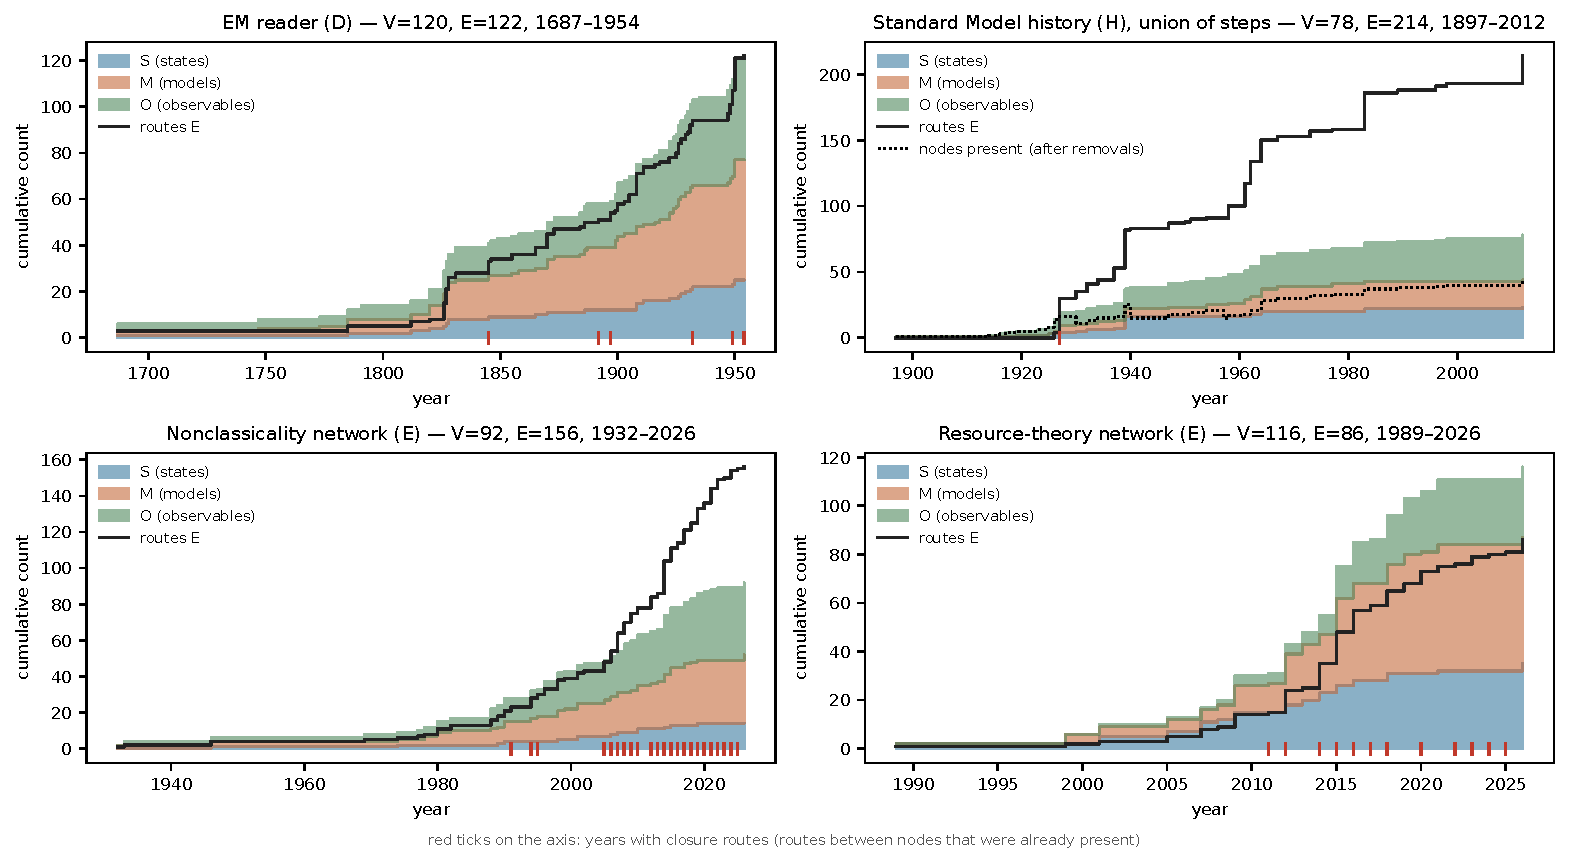
\includegraphics[width=\textwidth]{fig_evo_branches.pdf}
\caption{Cumulative node counts by layer (stacked) and route counts of the four branches on the calendar axis of \cref{def:dating}. Red ticks: years with closure routes. For the history the dotted line is the number of nodes present after removals (\cref{sec:removals}).}\label{fig:evo_branches}
\end{figure}

\begin{figure}[htbp]\centering
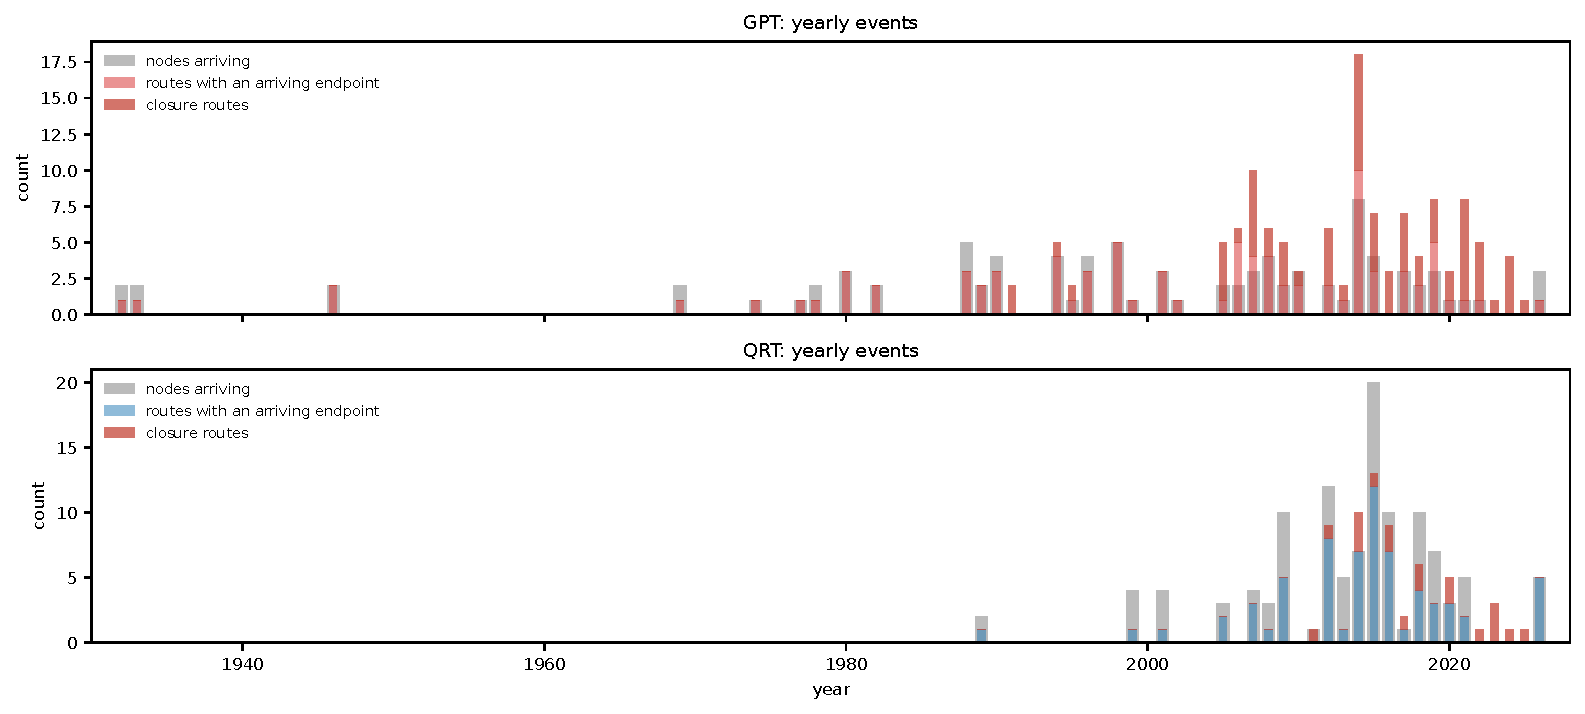
\includegraphics[width=\textwidth]{fig_evo_events.pdf}
\caption{Yearly events of the nonclassicality (GPT) and resource-theory (QRT) networks: nodes arriving, routes with an arriving endpoint, and closure routes.}\label{fig:evo_events}
\end{figure}

\subsection{The nonclassicality network}
The dated network starts with two nodes in \EGPTYZero{}: the complex-structure axiom and the quantum model (Stone's theorem, cited by \id{GN7}), then the Kirkwood--Dirac witness and effect (1933), the Moyal axiom and the Wigner-negative cluster (1946), the Bell witness and effect (1969), Gaussian states (1974) and the Wigner witness (1977). By 1950 the graph has \EGPTVAtOneNineFiveZero{} nodes and \EGPTEAtOneNineFiveZero{} routes, by 1980 \EGPTVAtOneNineEightZero{}/\EGPTEAtOneNineEightZero{}, by 1990 \EGPTVAtOneNineNineZero{}/\EGPTEAtOneNineNineZero{}, by 2000 \EGPTVAtTwoZeroZeroZero{}/\EGPTEAtTwoZeroZeroZero{}, by 2010 \EGPTVAtTwoZeroOneZero{}/\EGPTEAtTwoZeroOneZero{}, by 2020 \EGPTVAtTwoZeroTwoZero{}/\EGPTEAtTwoZeroTwoZero{}, and \EGPTVfin{}/\EGPTEfin{} at 2026. The route count overtakes the node count in \EGPTEoverV{} (\cref{fig:evo_branches}): \EGPTClosures{} of the \EGPTEfin{} routes (\EGPTClosureFrac\%) are closures, with mean latency \EGPTLatMean{} years, median \EGPTLatMedian{}, maximum \EGPTLatMax{}. This is the census-and-closure loop of \cref{ch:explore} seen in historical time: the cells of the witness matrix are opened by the arrival of witnesses and effects and are settled, on the median, fourteen years later. The per-year log of nodes and routes is \cref{app:events} (\cref{tab:evo_events_gpt}).

\paragraph{Witness before effect?} The \EgptPairs{} witness--effect pairs of the network (\cref{tab:evo_witness}) are dated the same year in \EgptPairsSame{} cases, the effect first in \EgptPairsEfirst{}, the witness first in \EgptPairsWfirst{}. Under the latest-source convention the counts are \EgptMaxPairsSame{}/\EgptMaxPairsEfirst{}/\EgptMaxPairsWfirst{}. In the data, therefore, a witness is never recorded before its effect except once, and most often the two appear in the same source: the effect is defined by the functional that detects it.

\paragraph{Explanation lag.} For each effect node, the years from its appearance to its first route from the model layer (\cref{tab:evo_explanation}): \EgptEffectsWithM{} of \EgptEffects{} effects have such a route, with mean lag \EgptLagMean{} years; \EgptLagZero{} are explained in their first year, Bell nonlocality waits \EgptLagBell{} years (\EgptBellYear{} to the first model route dated \EgptBellFirstM{}) and the Kirkwood--Dirac family \EgptLagKD{} years (\EgptKDYear{} to \EgptKDFirstM{}). The other \EgptEffectsNoM{} effects reach the model layer only through states or witnesses, which is the direct state--effect structure of type E (\cref{sec:contraction}).

\begin{table}[htbp]\centering\small
\caption{Witness--effect pairs of the nonclassicality network with the year of each member and of the pairing route.}\label{tab:evo_witness}
\begin{tabular}{@{}llrrrl@{}}\toprule
Witness & Effect & $t$(witness) & $t$(effect) & $t$(pair edge) & order \\\midrule
\texttt{w-bell} & \texttt{e-bell} & 1969 & 1969 & 1969 & same \\
\texttt{w-bell} & \texttt{e-pr} & 1969 & 1980 & 1994 & witness first \\
\texttt{w-steer} & \texttt{e-steer} & 2017 & 1998 & 2017 & effect first \\
\texttt{w-incomp} & \texttt{e-incomp} & 2019 & 1982 & 2019 & effect first \\
\texttt{w-entw} & \texttt{s-ent} & 1996 & 1989 & 1996 & effect first \\
\texttt{w-ncineq} & \texttt{e-ctx} & 2021 & 1989 & 2021 & effect first \\
\texttt{w-sic} & \texttt{e-ks} & 2008 & 1990 & 2008 & effect first \\
\texttt{w-kcbs} & \texttt{e-ksdep} & 2008 & 2008 & 2008 & same \\
\texttt{w-wig} & \texttt{s-wneg} & 1977 & 1946 & 1977 & effect first \\
\texttt{w-kd} & \texttt{e-kd} & 1933 & 1933 & 1933 & same \\
\texttt{w-weakval} & \texttt{e-weak} & 1988 & 1988 & 1988 & same \\
\texttt{w-workq} & \texttt{e-heat} & 2014 & 2014 & 2014 & same \\
\texttt{w-magicw} & \texttt{s-magic} & 2014 & 2001 & 2014 & effect first \\
\texttt{w-cohw} & \texttt{s-coh} & 2014 & 2007 & 2014 & effect first \\
\texttt{w-discw} & \texttt{s-discord} & 2008 & 2001 & 2008 & effect first \\
\texttt{w-clone} & \texttt{e-nobc} & 1996 & 1996 & 1996 & same \\
\texttt{w-vis} & \texttt{e-interf2} & 1988 & 1988 & 1988 & same \\
\texttt{w-sorkin} & \texttt{e-interf3} & 1994 & 1994 & 1994 & same \\
\bottomrule\end{tabular}

\end{table}

\begin{table}[htbp]\centering\small
\caption{Explanation lag of the effect nodes of the nonclassicality network: year of the effect, year of its first route from a model node and from a state node, and the lags.}\label{tab:evo_explanation}
\begin{tabular}{@{}lrrrrr@{}}\toprule
Effect & $t$(effect) & first M$\to$effect & lag (y) & first S$\to$effect & lag (y) \\\midrule
\texttt{e-kd} & 1933 & 1988 & 55 & 2021 & 88 \\
\texttt{e-bell} & 1969 & 1995 & 26 & 1989 & 20 \\
\texttt{e-pr} & 1980 & 1980 & 0 & -- & -- \\
\texttt{e-incomp} & 1982 & 1982 & 0 & -- & -- \\
\texttt{e-interf2} & 1988 & -- & -- & -- & -- \\
\texttt{e-weak} & 1988 & -- & -- & -- & -- \\
\texttt{e-ctx} & 1989 & 1990 & 1 & 1989 & 0 \\
\texttt{e-ks} & 1990 & -- & -- & 1990 & 0 \\
\texttt{e-interf3} & 1994 & 1994 & 0 & -- & -- \\
\texttt{e-nobc} & 1996 & -- & -- & 2008 & 12 \\
\texttt{e-steer} & 1998 & 1998 & 0 & -- & -- \\
\texttt{e-ksdep} & 2008 & -- & -- & 2014 & 6 \\
\texttt{e-heat} & 2014 & -- & -- & 2019 & 5 \\
\bottomrule\end{tabular}

\end{table}

\subsection{The resource-theory network}
The resource-theory network starts in \EQRTYZero{} with Werner's state and the nonlocality-free set, adds the convexity framework, discord (2001), magic (2005), entanglement and steering (2007) and the operation classes of 2009; the framework nodes (\id{F-QRT}, \id{F-TENSOR}) and five theories arrive in 2012, and the bulk of the network in 2014--2016 (by 2010 \EQRTVAtTwoZeroOneZero{} nodes, by 2015 \EQRTVAtTwoZeroOneFive{}, by 2020 \EQRTVAtTwoZeroTwoZero{}, \EQRTVfin{} at 2026). Here \EQRTClosures{} of \EQRTEfin{} routes (\EQRTClosureFrac\%) are closures with median latency \EQRTLatMedian{} years: the resource theories were connected to each other within a few years of being defined. The degree at arrival is low (\EQRTMeanArrDeg{} on average; \EQRTArrDegZero{} of \EQRTVfin{} nodes arrive with no route dated their own year), because a resource theory enters as a set of nodes (free set, resource set, operations, witness) whose routes are mostly the definitional ones that the data do not date and that the propagation rule places at the year of the latest endpoint.

\paragraph{The census in time.} \Cref{tab:evo_census} applies the pair census of \cref{ch:explore} to each year: the cells are the node pairs among the designated native-layer pairs (those that carry at least one edge in the final graph: \EgptDesignated{} pairs in GPT, \EqrtDesignated{} in QRT) restricted to the nodes present. The filled fraction of the nonclassicality network moves from \EGPTFilledRef\% in \EGPTFilledRefYear{} (\EGPTCellsRef{} cells) to \EGPTFilledLast\% in 2026 (\EgptCensusCellsFinal{} cells, a \EGPTCellsGrowth-fold growth); in the resource-theory network it falls from \EQRTFilledRef\% in \EQRTFilledRefYear{} to \EQRTFilledLast\% in 2026 (\EqrtCensusCellsFinal{} cells). The research front, measured as open cells, widens faster than it is filled, which is \cref{thm:agenda} read as a rate: the agenda grows quadratically in the node count while closures grow as $V^{\alpha}$ with $\alpha<2$ (\cref{sec:densification}).

\begin{table}[htbp]\centering\small
\caption{Pair census on the year axis: cells among present nodes in the designated layer pairs, connected cells, open cells and the filled fraction, at milestone years.}\label{tab:evo_census}
\begin{tabular}{@{}lrrrrr@{}}\toprule
Branch & Year & cells & connected & open & filled \\\midrule
GPT & 1990 & 295 & 21 & 274 & 7.1\% \\
GPT & 2005 & 868 & 45 & 823 & 5.2\% \\
GPT & 2010 & 1421 & 75 & 1346 & 5.3\% \\
GPT & 2015 & 2107 & 106 & 2001 & 5.0\% \\
GPT & 2020 & 2532 & 126 & 2406 & 5.0\% \\
GPT & 2026 & 2754 & 137 & 2617 & 5.0\% \\
QRT & 2005 & 78 & 5 & 73 & 6.4\% \\
QRT & 2015 & 2775 & 47 & 2728 & 1.7\% \\
QRT & 2020 & 5565 & 70 & 5495 & 1.3\% \\
QRT & 2026 & 6670 & 83 & 6587 & 1.2\% \\
\bottomrule\end{tabular}

\end{table}

\subsection{Polarity in time}
\Cref{fig:evo_polarity} separates the routes by polarity. The no-go routes of the nonclassicality network appear from \EGPTFirstNoGo{} and grow in step with the structural and possibility routes; in the resource-theory network the possibility routes (conversions, activations) dominate. \Cref{tab:evo_first_polarity} records, for each node, the polarity of its first incident route: \EgptMnoGoFirst{} of the \EgptMtotal{} model nodes of GPT enter through a pure no-go route and \EgptMnoGoAny{} through a first route that includes a no-go: a model (subtheory) is typically introduced by what it cannot do.

\begin{figure}[htbp]\centering
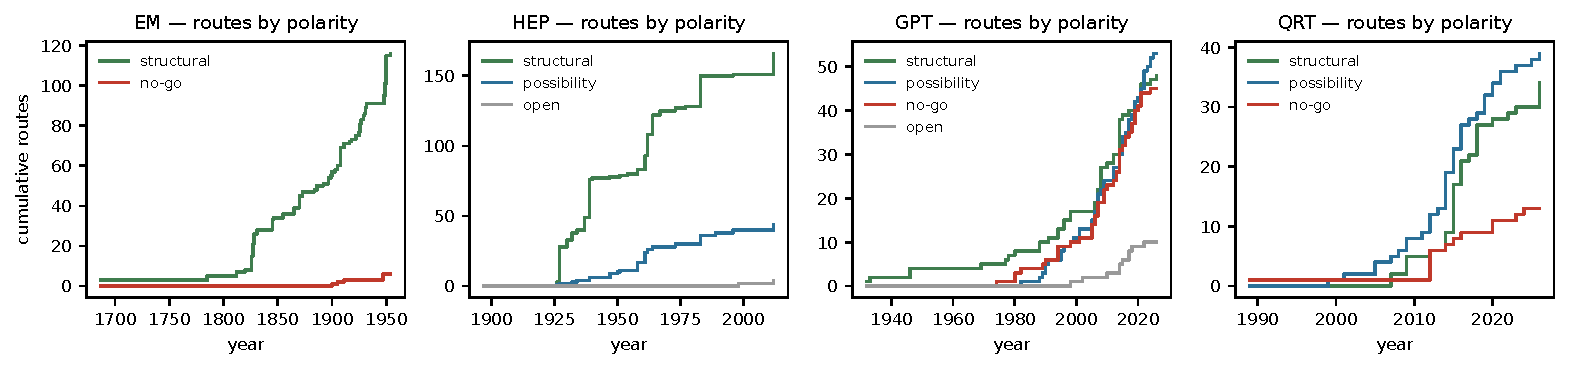
\includegraphics[width=\textwidth]{fig_evo_polarity.pdf}
\caption{Cumulative route counts by polarity. The reader's no-go routes are its failed derivations (R12); the history's possibility routes are its predictions and candidate routes; the effect networks separate structural, possibility and no-go closures.}\label{fig:evo_polarity}
\end{figure}

\begin{table}[htbp]\centering\small
\caption{Polarity of the first incident route of each node, by layer and branch (a node whose first routes have several polarities is counted under their combination; \emph{isolated} = no route).}\label{tab:evo_first_polarity}
\begin{tabular}{@{}l>{\raggedright\arraybackslash}p{3.6cm}>{\raggedright\arraybackslash}p{4.6cm}>{\raggedright\arraybackslash}p{4.2cm}@{}}\toprule
Branch & S nodes & M nodes & O nodes \\\midrule
EM & structural 24, no-go 1 (25) & structural 50, no-go 2 (52) & structural 38, no-go+\allowbreak{}structural 3, no-go 2 (43) \\
HEP & structural 22, open+\allowbreak{}structural 1 (23) & structural 12, possibility+\allowbreak{}structural 9 (21) & possibility 15, structural 14, possibility+\allowbreak{}structural 4, open 1 (34) \\
GPT & no-go 4, structural 3, no-go+\allowbreak{}possibility 2, no-go+\allowbreak{}structural 2, possibility 2, open+\allowbreak{}structural 1 (14) & no-go 17, structural 8, possibility 5, no-go+\allowbreak{}structural 2, no-go+\allowbreak{}possibility 2, isolated 2, no-go+\allowbreak{}possibility+\allowbreak{}structural 1, possibility+\allowbreak{}structural 1 (38) & structural 23, possibility 11, no-go 2, no-go+\allowbreak{}possibility 1, possibility+\allowbreak{}structural 1, no-go+\allowbreak{}structural 1, open 1 (40) \\
QRT & possibility 13, structural 12, isolated 3, no-go 3, possibility+\allowbreak{}structural 2, no-go+\allowbreak{}possibility+\allowbreak{}structural 1, no-go+\allowbreak{}structural 1 (35) & structural 20, possibility 11, isolated 9, no-go 8, no-go+\allowbreak{}structural 2, no-go+\allowbreak{}possibility 1, possibility+\allowbreak{}structural 1 (52) & possibility 14, isolated 13, structural 1, no-go 1 (29) \\
\bottomrule\end{tabular}

\end{table}

%=====================================================================
\chapter{The four-branch evolutionary network}\label{ch:merged}

\section{Construction}
\begin{definition}[evolutionary network]\label{def:merged}
Let $G_b$, $b\in\{\mathrm{EM},\mathrm{HEP},\mathrm{GPT},\mathrm{QRT}\}$, be the four dated graphs, where $G_{\mathrm{HEP}}$ is the \emph{union} of the twelve step graphs (every node and route that is drawn in any step, keyed by kind, inputs and target, dated at its first step and carrying the step at which it is last drawn), together with the observable-family, cluster-lineage and cluster-membership routes of the final view, dated at the year of their later endpoint. The evolutionary network at year $T$ is
\[ \mathcal G_T=\Bigl(\bigsqcup_b G_b\big|_{\le T}\Bigr)\cup\mathrm{Glue}_T, \]
where $G_b|_{\le T}$ keeps the nodes and routes with $t\le T$ (and, in HEP, drops an item once $T$ exceeds its removal year), and $\mathrm{Glue}_T$ contains, for each shared concept $c$ of the gluing catalogue (\cref{app:concepts}) with $k_c(T)\ge2$ members present, $k_c(T)-1$ identification edges joining its members in order of year. The \emph{collapsed} node count is $V^{\mathrm{col}}(T)=V(T)-\sum_c (k_c(T)-1)^+$, the number of nodes of the quotient of $\mathcal G_T$ by the identifications.
\end{definition}
\begin{lemma}\label{lem:collapse}
$V^{\mathrm{col}}(T)$ is the number of nodes of $\mathcal G_T/\!\sim$, where $u\sim v$ iff $u,v$ are members of the same concept, and $V^{\mathrm{col}}$ is non-decreasing in $T$ outside the HEP removal years.
\end{lemma}
\begin{proof}
The identification edges of a concept form a path on its $k_c$ present members, so the quotient merges them into one node and removes $k_c-1$ nodes; concepts are disjoint sets of members, so the removals add. Between removal years every term of $V(T)$ and every $k_c(T)$ is non-decreasing, and $V-\sum_c(k_c-1)^+=\sum_c 1+|\{v:\ v\text{ in no concept}\}|$ over present items is a count of present equivalence classes.
\end{proof}
The HEP union is the only non-monotone part of $\mathcal G_T$: \EhepRemovedNodes{} of its \EHEPVfin{} nodes and \EhepRemovedRoutes{} of its \EhepUnionRoutes{} routes are removed at some step (\cref{sec:removals}). A removal is placed at the start year of the removing step, never before the item's own year, and the final view (step 12, ``1927--2012'') places its removals at 2012. The merged curves of this chapter count ever-added items; the removal toggle of the explorer page and the dotted line of \cref{fig:evo_branches} apply the removals.

\section{Growth of the merged network}
\begin{figure}[htbp]\centering
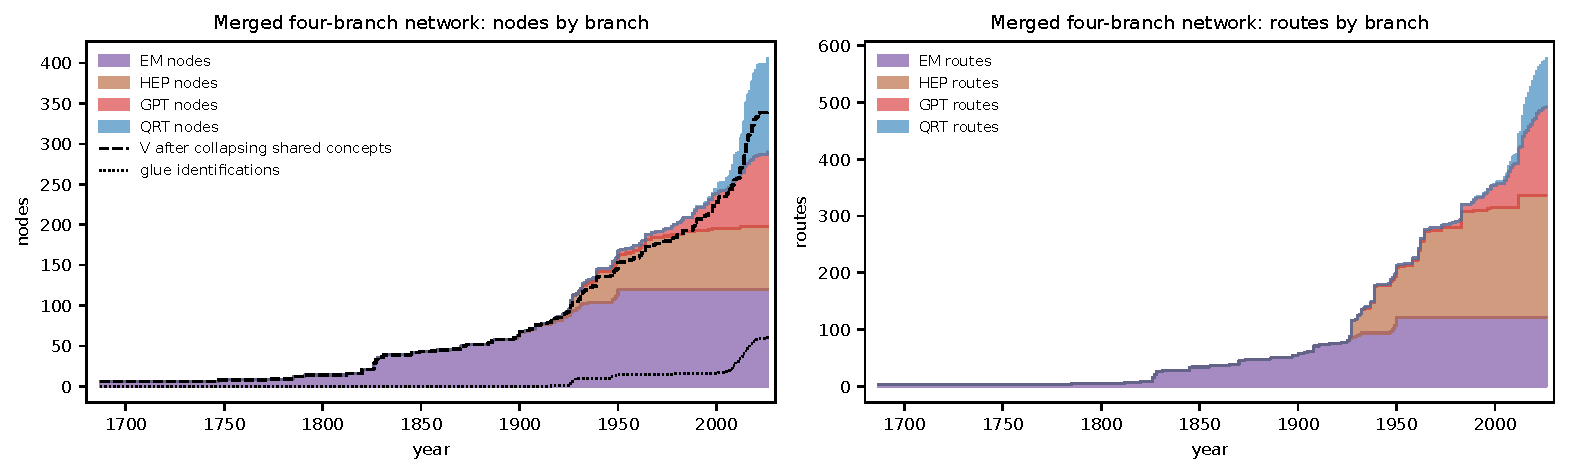
\includegraphics[width=\textwidth]{fig_evo_merged.pdf}\\[4pt]
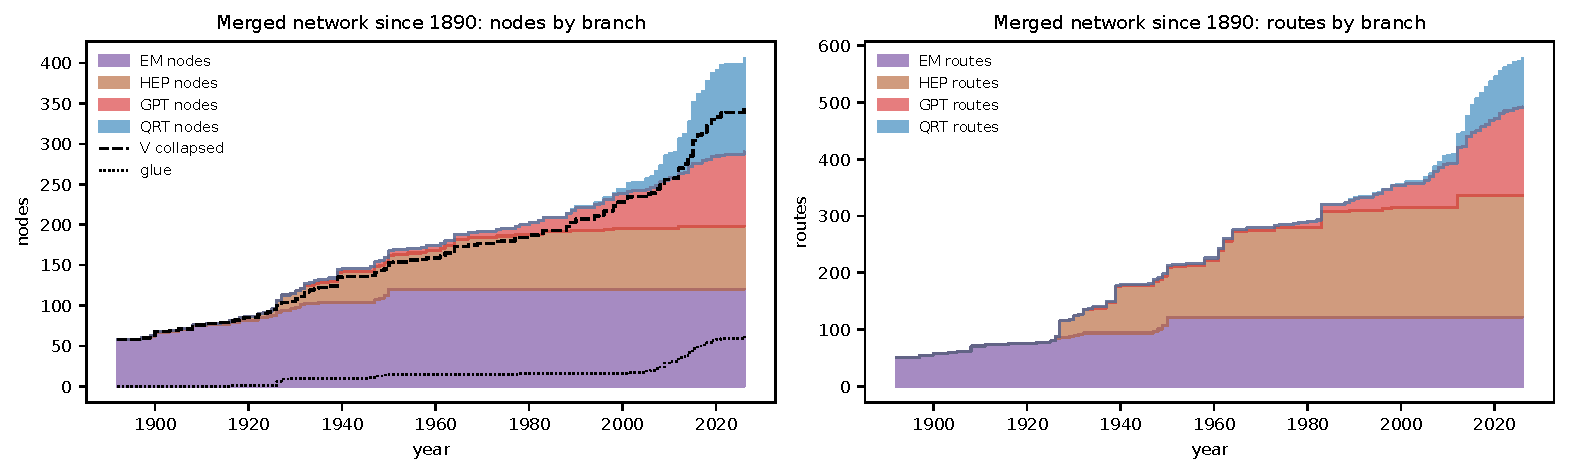
\includegraphics[width=\textwidth]{fig_evo_merged_zoom.pdf}
\caption{The evolutionary network: nodes (left) and routes (right) by branch, stacked, with the collapsed node count and the number of glue identifications; full axis above, from 1890 below.}\label{fig:evo_merged}
\end{figure}
At 1900 the evolutionary network has \EmergedVAtOneNineZeroZero{} nodes and \EmergedEAtOneNineZeroZero{} routes, all from the electromagnetism reader, and no glue; at 1950, \EmergedVAtOneNineFiveZero{} nodes, \EmergedEAtOneNineFiveZero{} routes and \EmergedGlueAtOneNineFiveZero{} identifications (the EM--HEP overlap of the 1920s--1940s: Lagrangian, photon, fine-structure constant, Lamb shift, anomalous moment); at 2000, \EmergedVAtTwoZeroZeroZero{}/\EmergedEAtTwoZeroZeroZero{}/\EmergedGlueAtTwoZeroZeroZero{}; at 2026, \EmergedV{} nodes (S \EmergedS{}, M \EmergedM{}, O \EmergedO{}), \EmergedE{} routes, \EmergedGlue{} identifications over \EnSharedFour{} shared concepts and \EmergedVcollapsed{} collapsed nodes. Half of the final node count is reached in \EmergedHalfYear{} and half of the final route count in \EmergedHalfYearE{}: the network of these four branches is, by count, a late-twentieth-century object, because the two effect networks are. \Cref{fig:evo_lanes} draws every node at its year in four lanes.

\begin{figure}[htbp]\centering
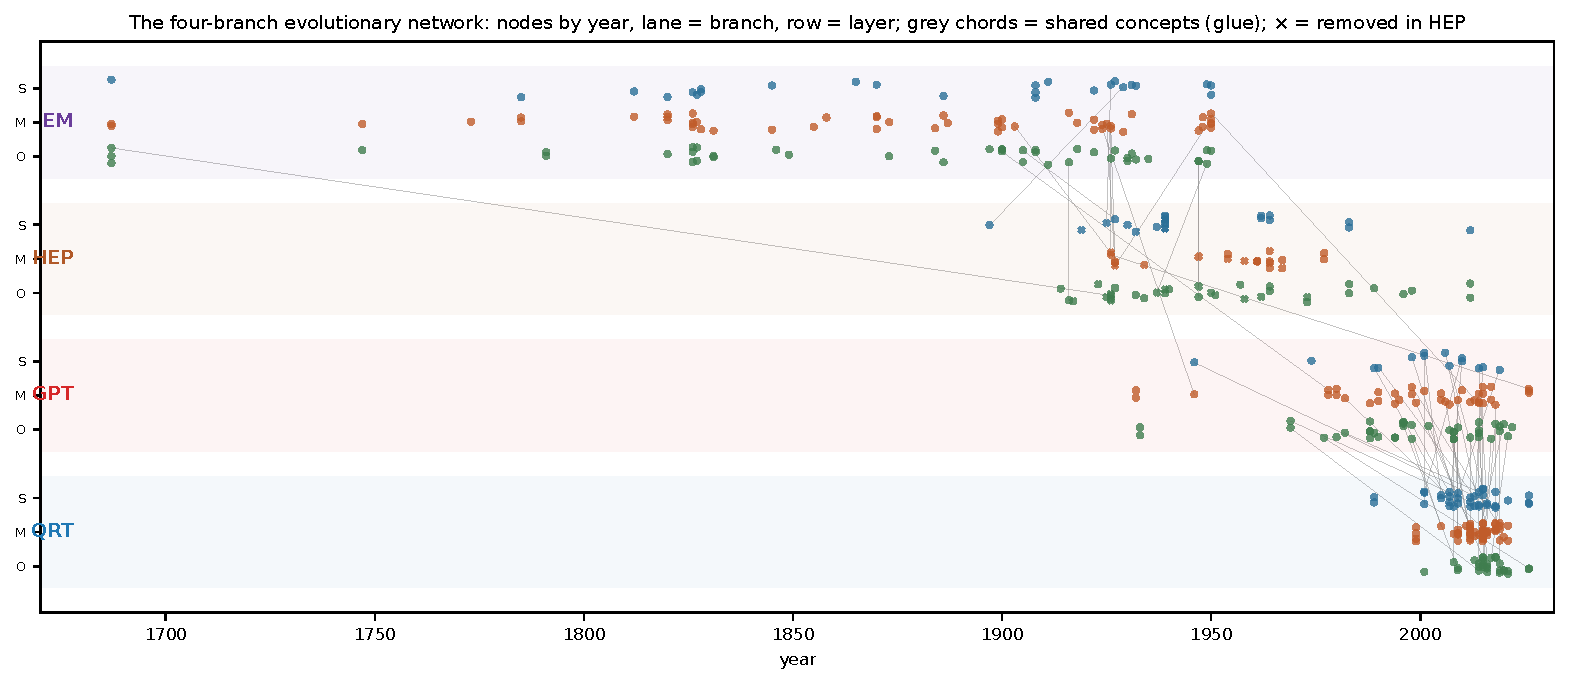
\includegraphics[width=\textwidth]{fig_evo_lanes.pdf}
\caption{Every node of the evolutionary network at its year (lane = branch, row = layer, colour = layer); grey chords join the members of shared concepts across branches; $\times$ marks nodes removed in the history.}\label{fig:evo_lanes}
\end{figure}

\section{Transfer between branches}\label{sec:transfer}
A shared concept has a year in each branch, and the \emph{lag} is the difference between the latest and earliest of them over its dated members (\cref{tab:evo_concepts_lag}, \cref{fig:evo_concepts}). Over the \EnSharedDated{} dated shared concepts the mean lag is \ElagMean{} years, the median \ElagMedian{}, \ElagZero{} are simultaneous and the maximum is \ElagMax{} (\ElagMaxLabel{}: \ElagMaxYears{}; in the history it is the position operator of one-particle quantum mechanics). The direction of transfer:
\begin{itemize}[nosep]
\item Between the two effect networks (\EnSharedGPTQRT{} shared concepts): GPT precedes QRT in \EfirstGPTamongGQ{} (mean lag \ElagGPTfirstMean{} years), QRT precedes in \EfirstQRTamongGQ{} (mean lag \ElagQRTfirstMean{} years), \EtieGQ{} are simultaneous. The dominant direction agrees with the contraction lemma of \cref{sec:contraction} read in time: an effect is named, witnessed and connected to subtheories before its state cluster is made the resource set of a resource theory.
\item Between the reader and the history (\EnSharedEMHEP{} shared concepts): EM first in \EfirstEMamongEH{}, HEP first in \EfirstHEPamongEH{}, \EtieEH{} simultaneous. The reader reaches the QED-era concepts (the electron field, the QED interaction, the cross section) later than the history dates them, because the reader's year is that of its paragraph while the history's is the node's own year field.
\end{itemize}
One shared concept (\EnSharedUndated{}) has a project-dated member in one branch and no dated lag. The lags inherit the ingredient-chronology caveat of \cref{sec:dating-caveat}; what the caveat cannot change is the simultaneous cases and the direction of a lag of a decade or more.

\begin{figure}[htbp]\centering
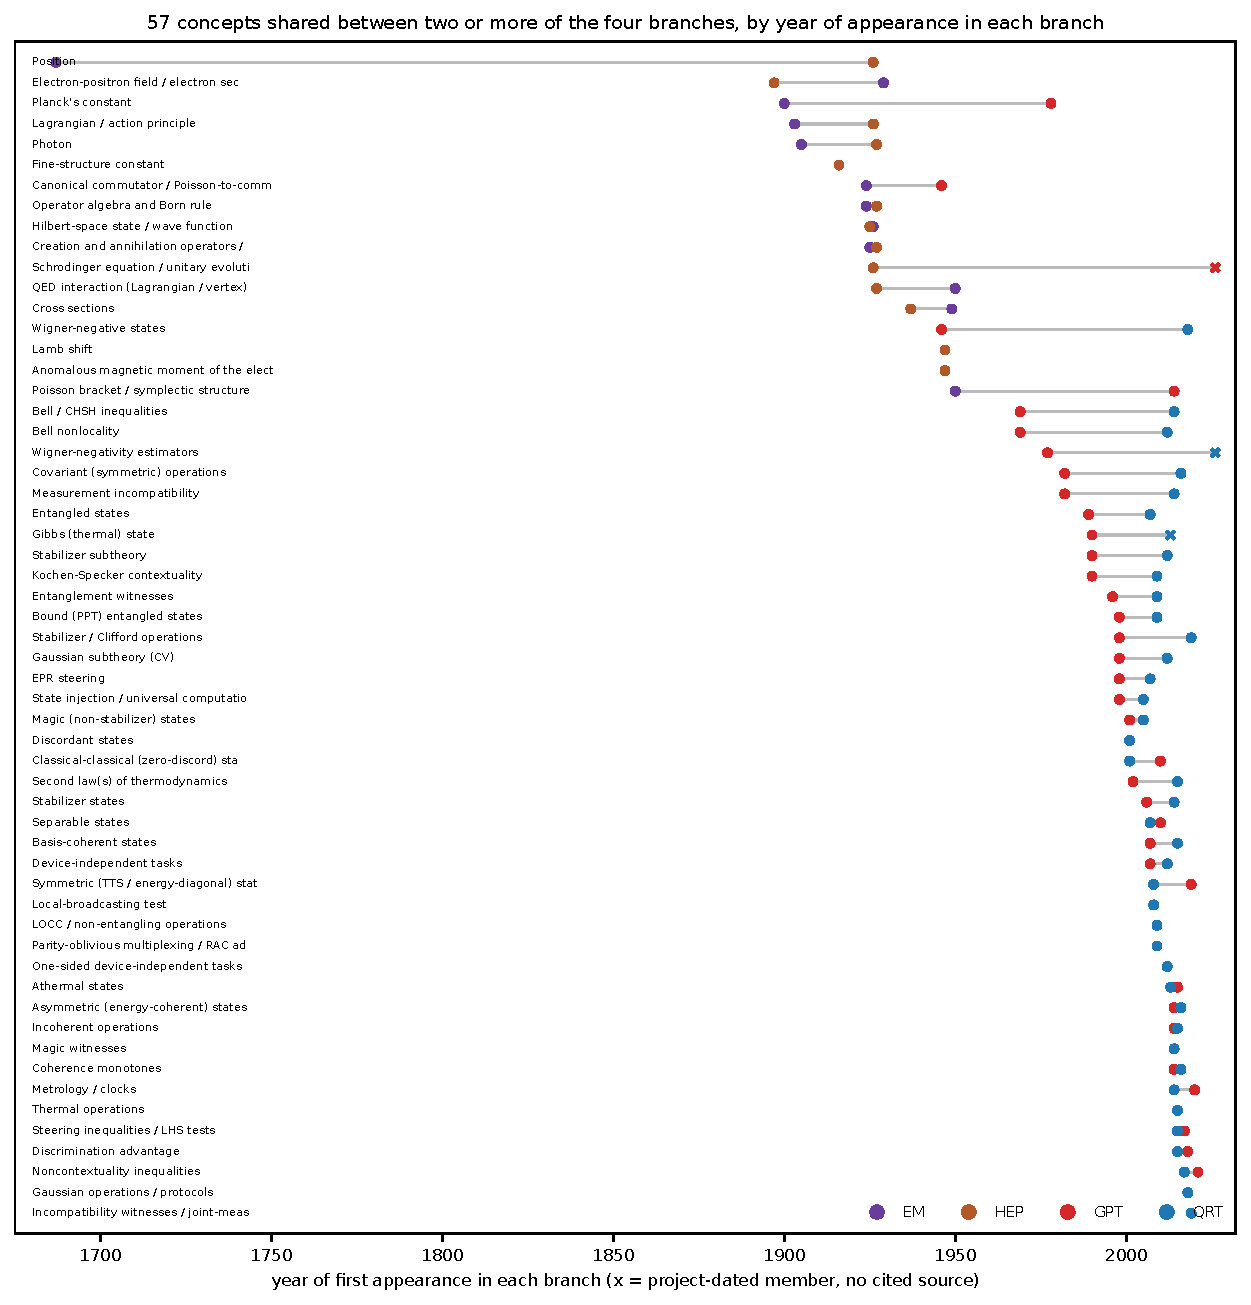
\includegraphics[width=\textwidth]{fig_evo_concepts.pdf}
\caption{The \EnSharedFour{} shared concepts of the four branches by year of first appearance in each branch (colour = branch; $\times$ = project-dated member).}\label{fig:evo_concepts}
\end{figure}

%=====================================================================
\chapter{Growth rules and counting identities}\label{ch:growth}

\section{The counting identity}
\begin{theorem}[arrival--closure identity]\label{thm:identity}
In a dated graph with $E$ routes, let $a(r)$ be the number of endpoints of $r$ with $t(u)=t(r)$, and let $C$ be the number of closure routes ($a(r)=0$). Then
\[ E=\sum_{v}d_{\mathrm{arr}}(v)-\sum_{r}\bigl(a(r)-1\bigr)^{+}+C . \]
\end{theorem}
\begin{proof}
$\sum_v d_{\mathrm{arr}}(v)=\sum_r a(r)$ by double counting the pairs $(v,r)$ with $v\in r$ and $t(v)=t(r)$. A route with $a(r)\ge1$ contributes $a(r)=1+(a(r)-1)^+$ to this sum and a route with $a(r)=0$ contributes $0$; so $\sum_r a(r)-\sum_r(a(r)-1)^+=|\{r:a(r)\ge1\}|=E-C$.
\end{proof}
The correction term is non-zero exactly for routes whose endpoints arrive together, which in a graph of directed hyperedges is common: a derivation of the reader that introduces its target together with one of its inputs, an \id{enters} route of the history dated with the sector it enters. \Cref{tab:evo_identity} verifies the identity on the four branches; it is the temporal counterpart of the count deltas of \cref{tab:ops}: every operation of Part I either adds a node with $d_{\mathrm{arr}}$ routes, adds a closure route, or removes.
\begin{table}[htbp]\centering\small
\caption{The arrival--closure identity of \cref{thm:identity} on the four dated branches.}\label{tab:evo_identity}
\begin{tabular}{@{}lrrrrrl@{}}\toprule
Branch & $\sum_v d_{\mathrm{arr}}(v)$ & $\sum_r (a(r)-1)^+$ & closures & $\sum_v d_{\mathrm{arr}} - \sum_r (a(r)-1)^+ + \text{closures}$ & $E$ & holds \\\midrule
EM & 174 & 60 & 8 & 122 & 122 & yes \\
HEP & 234 & 24 & 4 & 214 & 214 & yes \\
GPT & 110 & 23 & 69 & 156 & 156 & yes \\
QRT & 87 & 20 & 19 & 86 & 86 & yes \\
\bottomrule\end{tabular}

\end{table}

\begin{table}[htbp]\centering\small
\caption{Growth summary of the four dated branches. Frac.: closure fraction $C/E$. $\bar d_{\mathrm{arr}}$: mean degree at arrival. $\alpha$ ($R^2$): densification fit $\log E=\alpha\log V+c$ over the filtration years with $V\ge10$. PA ratio: mean degree of the endpoints of closure routes over the mean degree of all nodes present, evaluated before each closure ($n$ = number of closures).}\label{tab:evo_summary}
\resizebox{\textwidth}{!}{\begin{tabular}{@{}llrrrrrlrll@{}}\toprule
Branch & Years & $V$ & S/M/O & $E$ & Closures & Frac. & Latency mean/med/max (y) & $\bar d_{\mathrm{arr}}$ & $\alpha$ ($R^2$) & PA ratio ($n$) \\\midrule
EM & 1687--1954 & 120 & 25/52/43 & 122 & 8 & 7\% & 23.8 / 17 / 77 & 1.45 & 1.40 (0.98) & 1.16 (8) \\
HEP & 1897--2012 & 78 & 23/21/34 & 214 & 4 & 2\% & 1.0 / 1 / 1 & 3.00 & 1.62 (0.87) & 3.56 (4) \\
GPT & 1932--2026 & 92 & 14/38/40 & 156 & 69 & 44\% & 15.7 / 14 / 41 & 1.20 & 1.47 (0.99) & 2.86 (69) \\
QRT & 1989--2026 & 116 & 35/52/29 & 86 & 19 & 22\% & 4.1 / 4 / 12 & 0.75 & 1.30 (1.00) & 1.71 (19) \\
\bottomrule\end{tabular}
}
\end{table}

\section{Arrival degree and closure latency}
\Cref{tab:evo_summary} collects the quantities per branch. The mean degree at arrival separates the branch types: the history's nodes arrive with \EHEPMeanArrDeg{} routes each (a new sector enters its model and its observables in the same step), the reader's with \EEMMeanArrDeg{}, the effect networks' with \EGPTMeanArrDeg{} and \EQRTMeanArrDeg{}. The closure fraction is the complementary quantity: \EEMClosureFrac\% in the reader, \EHEPClosureFrac\% in the history, \EGPTClosureFrac\% and \EQRTClosureFrac\% in the effect networks. The readers and the history are \emph{arrival-driven}: a route almost always enters with a node, because a paragraph derives a new result and a step draws a new sector. The effect networks are \emph{closure-driven} to a large degree: their routes are theorems between existing nodes. \Cref{fig:evo_latency} gives the latency distributions: the reader's \EEMClosures{} closures have mean latency \EEMLatMean{} years (the two longest, \EEMLatSecond{} and \EEMLatMax{} years, are the Lorentz-force derivations of the 1890s between charge, force and field nodes of the 1820s), the history's \EHEPClosures{} closures have latency \EHEPLatMean{}, the effect networks' \EGPTLatMean{} and \EQRTLatMean{}.
\begin{figure}[htbp]\centering
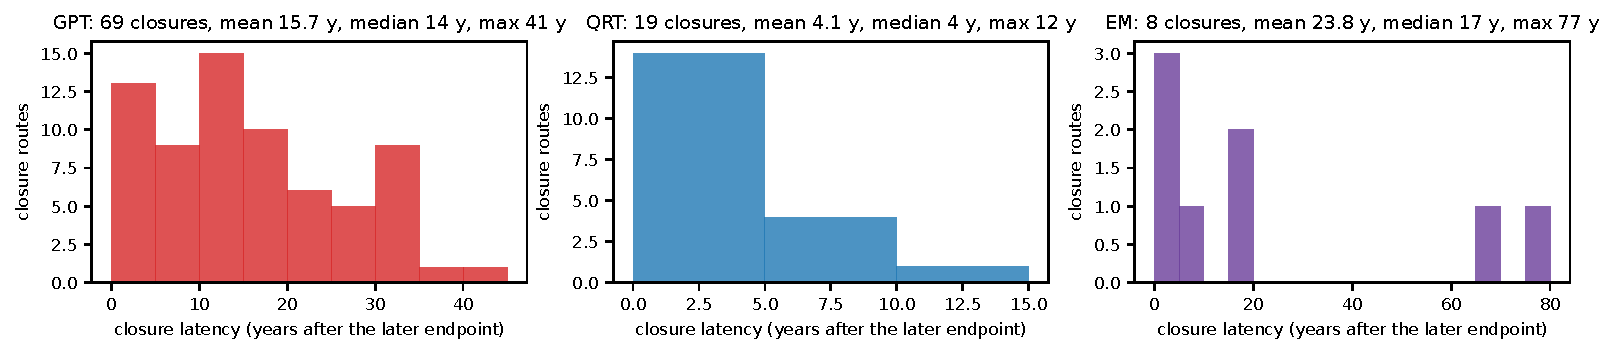
\includegraphics[width=\textwidth]{fig_evo_latency.pdf}
\caption{Closure latency (years from the later endpoint to the closure route) in the three branches with more than four closures.}\label{fig:evo_latency}
\end{figure}

\section{Preferential closure}\label{sec:pa}
For each closure route, the engine compares the mean degree of its endpoints at that time with the mean degree of all nodes then present; the ratio of the two sums over all closures is the \emph{preferential-closure ratio}, a discrete form of the attachment-kernel test of preferential-attachment models \citep{barabasi1999,newman2001}. It is \EGPTPAratio{} in GPT (\EGPTPAn{} closures), \EQRTPAratio{} in QRT (\EQRTPAn{}), \EEMPAratio{} in EM (\EEMPAn{}); the history has \EHEPPAn{} closures and the ratio is not meaningful. Closures attach to the best-connected nodes present: in the nonclassicality network the endpoints of a closing theorem have almost three times the mean degree. This is the behaviour of the census loop when the solver is the literature: the cells adjacent to well-studied nodes (Bell nonlocality, entanglement, Wigner negativity) are the ones for which a theorem is found.

\section{Densification}\label{sec:densification}
On the year filtration the route count grows faster than the node count. Fitting $\log E(T)=\alpha\log V(T)+c$ over the filtration years with $V(T)\ge10$ (\cref{fig:evo_densification}) gives $\alpha=\EEMAlpha{}$ ($R^2=\EEMAlphaR$) for the reader, \EHEPAlpha{} (\EHEPAlphaR) for the history, \EGPTAlpha{} (\EGPTAlphaR) for the nonclassicality network and \EQRTAlpha{} (\EQRTAlphaR) for the resource-theory network. Exponents between 1 and 2 are the densification power law observed in citation and collaboration graphs \citep{leskovec2007}; here they hold for concept graphs whose edges are mathematical relations, and they are stable under the dating convention (\cref{tab:evo_robust}). The right panel of \cref{fig:evo_densification} shows the degree-at-arrival distributions.
\begin{figure}[htbp]\centering
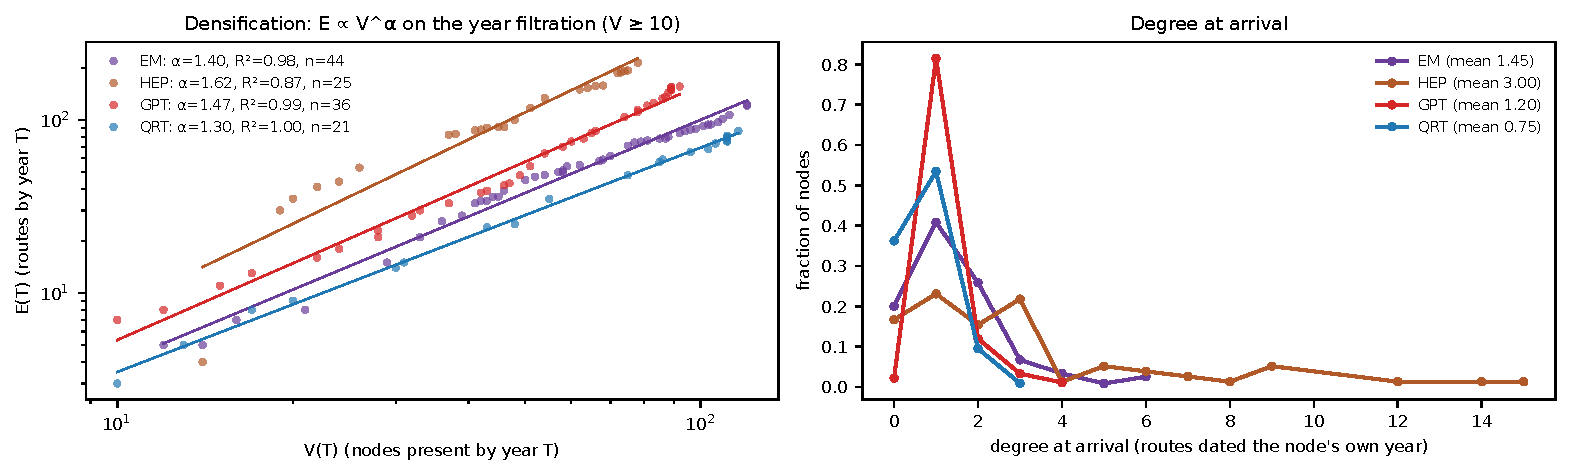
\includegraphics[width=\textwidth]{fig_evo_densification.pdf}
\caption{Left: $E(T)$ against $V(T)$ on the year filtration (log--log) with the fitted power laws. Right: distribution of the degree at arrival.}\label{fig:evo_densification}
\end{figure}

\section{Removals: the history as the only non-monotone branch}\label{sec:removals}
The reader and the two effect networks are filtrations: nothing is removed. The Standard Model history removes. \Cref{tab:evo_hep_removals} and \cref{fig:evo_hep_removals} count, per step, the nodes and routes added and removed in the union graph: \EhepRemovedNodes{} of \EHEPVfin{} nodes and \EhepRemovedRoutes{} of \EhepUnionRoutes{} routes. By sub-layer, the removed nodes are \EhepOdirectRemoved{} of \EhepOdirectAll{} direct observables (an observable is drawn in the step that explains it and dropped from the next drawing), \EhepSuirRemoved{} of \EhepSuirAll{} unitary-irreducible-representation state nodes (the Wigner classification of step 2, re-partitioned into Fock space and sectors at step 4), \EhepMfundRemoved{} of \EhepMfundAll{} fundamental model nodes (absorbed into the Lagrangian clusters of the final view), \EhepMeffRemoved{} of \EhepMeffAll{} effective models and \EhepMcandRemoved{} of \EhepMcandAll{} candidate (Fermi, muon and $V\!-\!A$ contact terms absorbed by their successors, R7/R10), \EhepSsectorRemoved{} of \EhepSsectorAll{} sectors and \EhepMframeRemoved{} of \EhepMframeAll{} frames; the \EhepMclusterAll{} cluster nodes are never removed. Removal in the history is of two kinds that the data distinguish: \emph{absorption}, where a lineage or back-edge names the successor, and \emph{de-selection}, where the page stops drawing an observable that is still explained. Only the first changes the state of knowledge; the cumulative view of \cref{ch:hep} keeps de-selected observables, and \cref{def:merged} keeps both with their removal step so that either reading can be reconstructed.
\begin{table}[htbp]\centering\small
\caption{Additions and removals per step of the Standard Model history (union graph).}\label{tab:evo_hep_removals}
\resizebox{\textwidth}{!}{\begin{tabular}{@{}lrrrrp{6.2cm}@{}}\toprule
Step & nodes added & routes added & nodes removed & routes removed & nodes removed (native ids) \\\midrule
1 & 9 & 9 & 0 & 0 &  \\
2 & 11 & 29 & 2 & 4 & H1, o\_x \\
3 & 1 & 0 & 1 & 1 & o\_L \\
4 & 8 & 37 & 14 & 31 & m\_L, o\_E, o\_p, o\_S, u\_vac, u\_m0, u\_mh, u\_m1, u\_0h, u\_01, u\_02, u\_cs, u\_tach, o\_prod \\
5 & 7 & 6 & 4 & 4 & o\_m, o\_s, o\_G, o\_sig \\
6 & 3 & 4 & 2 & 2 & o\_pair, o\_lamb \\
7 & 7 & 21 & 1 & 7 & s\_nu \\
8 & 3 & 11 & 2 & 8 & m\_fermi, m\_mu \\
9 & 13 & 37 & 8 & 23 & s\_p, s\_n, o\_compton, o\_ntau, o\_michel, o\_twonu, m\_va, o\_hel \\
10 & 8 & 15 & 1 & 7 & o\_sw \\
11 & 2 & 2 & 0 & 2 &  \\
12 & 6 & 43 & 8 & 22 & m\_qed, m\_cc, m\_nc, m\_gs, m\_hg, m\_yuk, m\_pot, m\_numass \\
\bottomrule\end{tabular}
}
\end{table}
\begin{figure}[htbp]\centering
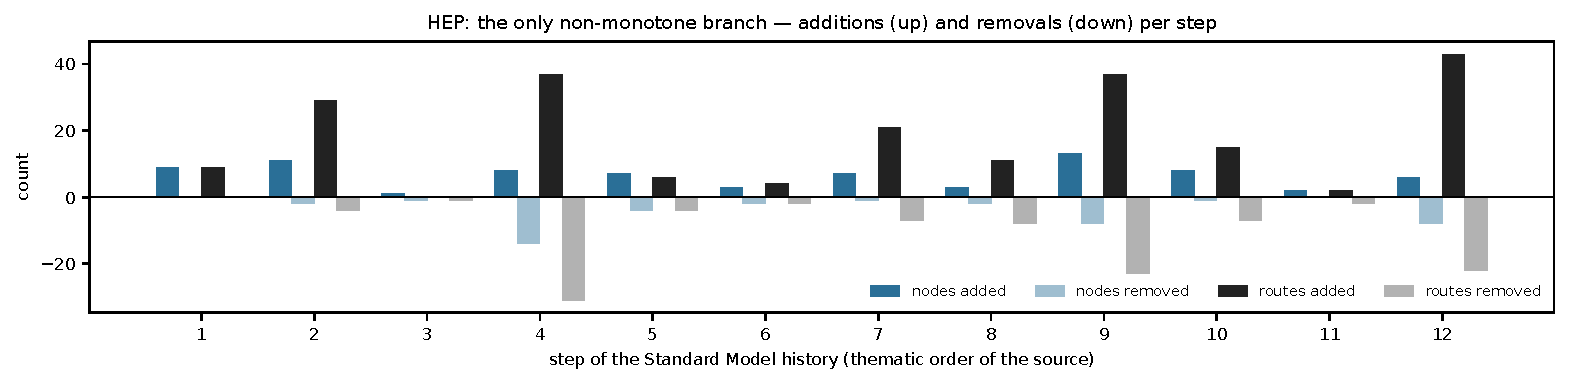
\includegraphics[width=\textwidth]{fig_evo_hep_removals.pdf}
\caption{Nodes and routes added (up) and removed (down) per step of the Standard Model history.}\label{fig:evo_hep_removals}
\end{figure}

\section{Rules on the year axis}\label{sec:rules-time}
Every route of the four branches is attributed to a rule of \cref{ch:rules}: in the reader, R11 (derive) or R12 (fail); in the history, by its kind (\id{enters} $\to$ R4, \id{predicts}/\id{frames}/\id{candidate} $\to$ R2, \id{calibrates} $\to$ R9, \id{backedge} $\to$ R1/R3, \id{lineage} $\to$ R7/R10, \id{subset} $\to$ the observable-family coarse-graining); in the effect networks, R14 (closure) split by the polarity of the closing route, and R13 (open cell) for routes of open status. \Cref{tab:evo_rules_decade} counts the firings per decade and \cref{fig:evo_hep_rules} places the automatically detected rule firings of the Standard Model replay (\cref{sec:detection}) on the year axis.

The connection between the rules and the node and edge numbers is the identity of \cref{thm:identity} read rule by rule. With $\Delta V(T)$ the arrivals of year $T$ and $\Delta E(T)=\Delta E_{\mathrm{arr}}(T)+\Delta E_{\mathrm{clo}}(T)$ the arrival and closure routes:
\begin{itemize}[nosep]
\item R11 (derive) adds one route and $0$ to $k$ nodes; in the reader it contributes \EEMSumArrDeg{} arrival incidences over \EEMVfin{} nodes and only \EEMClosures{} closures, so $\Delta E_{\mathrm{arr}}$ carries the reader. R12 (fail) adds one no-go route with the same counts.
\item R4 (route) and R1/R3 (partition--extend) in the history add routes with their nodes ($\Delta V>0$, $\Delta E_{\mathrm{arr}}>0$); R2 (a model node for a flagged observable) adds a node and its routes; R9 (calibrate) adds a route between a model and an observable, dated in the data with the observable it calibrates and therefore an arrival route; the history's \EHEPClosures{} closures are the entry and back-edge routes of the electron and proton sectors into unitary evolution at the Fock-space step, dated one year after their endpoints; R7/R10 (absorb, cluster) remove: they are the negative terms of the history's curve.
\item R13 (open cell) adds no route and no node: it is the term of the agenda, not of $E$; its firings are the open-status routes the data record (\EgptCensusOpenFinal{} open cells remain in GPT at 2026 under the designated pairs). R14 (close) adds one route and no node in \EGPTClosures{} of \EGPTEfin{} GPT routes and \EQRTClosures{} of \EQRTEfin{} QRT routes; it is the closure term.
\end{itemize}
Hence $\Delta V$ is driven by R2, R4, R1/R3 and the arrivals of R11; $\Delta E_{\mathrm{clo}}$ by R14 (and, rarely, by R4/R1 routes dated after their endpoints and by the reader's late derivations); and the only negative deltas are R7/R10. The densification exponent summarises the balance: $\alpha>1$ in every branch because closures and multi-route arrivals add routes without nodes.

\begin{figure}[htbp]\centering
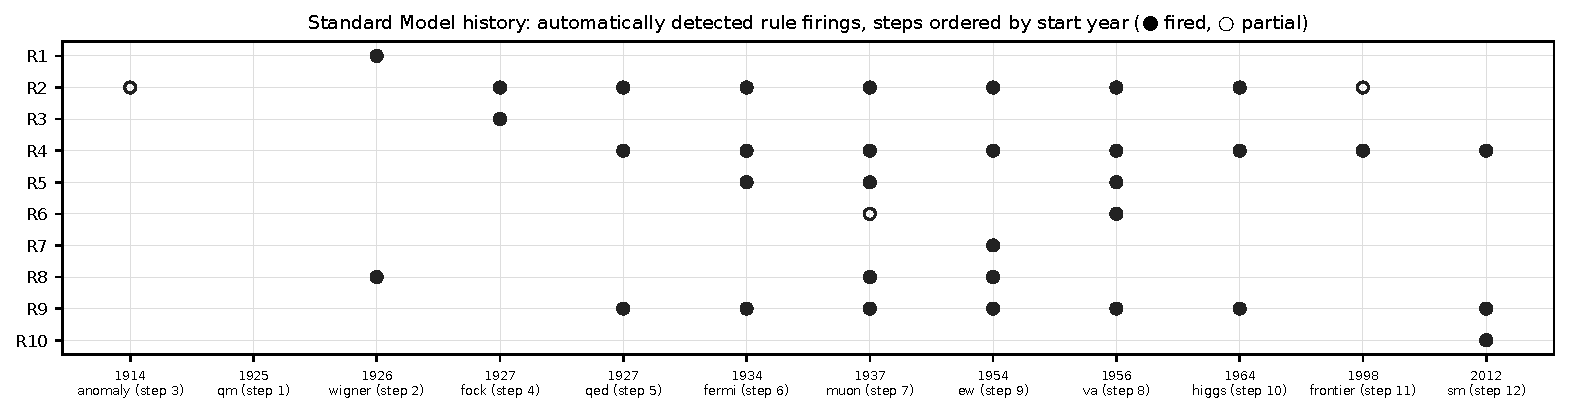
\includegraphics[width=\textwidth]{fig_evo_hep_rules.pdf}
\caption{Rule firings of the Standard Model history detected from structure (\cref{sec:detection}), with the steps ordered by their start year.}\label{fig:evo_hep_rules}
\end{figure}

\section{Temporal rules}\label{sec:te}
The following regularities are read off the dated data in the same spirit as R1--R10 were read off one history: they are stated so that a new branch can violate them.
\begin{description}[nosep]
\item[TE1 (arrival).] A node enters with its arrival routes, dated the same year; the mean degree at arrival is branch-specific (EM \EEMMeanArrDeg{}, HEP \EHEPMeanArrDeg{}, GPT \EGPTMeanArrDeg{}, QRT \EQRTMeanArrDeg{}) and is the dominant term of $E$ in the reader and the history.
\item[TE2 (closure).] In the effect networks a large share of routes are closures (GPT \EGPTClosureFrac\%, QRT \EQRTClosureFrac\%) with median latency \EGPTLatMedian{} and \EQRTLatMedian{} years: the census (R13) is worked off years after the nodes appear.
\item[TE3 (preferential closure).] Closures attach to nodes of above-average degree (ratios \EGPTPAratio{}, \EQRTPAratio{}, \EEMPAratio{}).
\item[TE4 (densification).] $E\propto V^{\alpha}$ with $1<\alpha<2$ in every branch (\EEMAlpha{}, \EHEPAlpha{}, \EGPTAlpha{}, \EQRTAlpha{}).
\item[TE5 (removal).] Only the history removes, by absorption into a successor or by the final clustering; the reader and the effect networks are monotone.
\item[TE6 (transfer).] A shared concept appears in a second branch with a lag (median \ElagMedian{} years); between the effect networks the dominant direction is effect network $\to$ resource network (\EfirstGPTamongGQ{} to \EfirstQRTamongGQ{}, \EtieGQ{} ties).
\end{description}

%=====================================================================
\chapter{The method in the evolution}\label{ch:method-time}

\section{Phases}
Part I named the loop observe $\to$ hypothesise $\to$ feed back $\to$ observe and wrote it as \cref{alg:step}. On the year axis each event of the four branches is assigned a \emph{phase} mechanically, by its layer (for a node) or its kind and status (for a route), as in \cref{tab:phase_map}. The assignment is the only hand-made element of this part, and it is a lookup table: no event is placed by reading its content.
\begin{table}[htbp]\centering\small
\caption{Phase assignment of events. A node arrival is assigned by its layer; a route by its universal kind, with open status overriding to \emph{deficit}.}\label{tab:phase_map}
\begin{tabular}{@{}lp{10.5cm}@{}}\toprule
Phase & Events \\\midrule
observe & O-node arrival; \id{witness}, \id{pairs} routes \\
deficit & routes of open status (R13 open cells) \\
hypothesize & M-node arrival; \id{frames}, \id{candidate}, \id{generates} \\
restructure & S-node arrival; \id{enters}, \id{backedge}, \id{member}, \id{satisfies} \\
predict & \id{derives}, \id{predicts}, \id{implies}, \id{necessary}, \id{enables}, \id{converts\_to}, \id{activates}, \id{reversible}, \id{hosts}, \id{bounds} \\
falsify & \id{failed}, \id{not\_implies}, \id{forbids}, \id{hides}, \id{excludes}, \id{distinct}, \id{violates}, \id{irreversible} \\
calibrate & \id{calibrates} \\
reduce & \id{lineage}, \id{subset}, \id{equiv}, \id{specializes}, \id{contains} \\
\bottomrule\end{tabular}
\end{table}

\Cref{tab:evo_merged_phases} and \cref{fig:evo_phases} count the \EphaseTotal{} events of the evolutionary network (\EmergedV{} arrivals and \EmergedE{} routes) by phase and decade: observe \Ephaseobserve{}, deficit \Ephasedeficit{}, hypothesize \Ephasehypothesize{}, restructure \Ephaserestructure{}, predict \Ephasepredict{}, falsify \Ephasefalsify{}, calibrate \Ephasecalibrate{}, reduce \Ephasereduce{}. Three readings of the table are supported by the counts.
\begin{enumerate}[nosep]
\item \emph{The phases run concurrently.} From the 1820s on, every decade with ten or more events (\EnBigDecades{} decades) contains at least \EminActivePhases{} phases, and the \EdecadesAllPhases{} contain all eight. The loop is not a sequence of eras; it is a cycle executed many times in parallel on different parts of the graph, which is what \cref{alg:step} does when it is run per event.
\item \emph{The branch types have phase profiles} (right panel of \cref{fig:evo_phases}). The reader is predict-heavy (derivations), the history restructure-heavy (sectors entering models, back-edges), the nonclassicality network falsify- and predict-heavy (theorems of both polarities), the resource-theory network observe- and hypothesize-heavy (witnesses and resource definitions). The profile is a consequence of the layer-pair signature of \cref{ch:types}: a type-D signature produces derivations, a type-H signature produces entries, a type-E signature produces closures.
\item \emph{Falsification is late and branch-specific.} The first falsify route of the reader is dated \EEMFirstFalsify{} (the classical derivations that fail at the quantum boundary), of the nonclassicality network \EGPTFirstFalsify{}, of the resource-theory network \EQRTFirstFalsify{} (its first no-go route, Werner's local model for entangled states, is a membership route dated 1989 and counts as restructure); the history has no falsify route, because in the data its refutations are recorded as removals and replacements (R7/R10, \cref{sec:removals}), not as routes. The decade with the most falsify events is the \EdecadeMaxfalsify{}s (\EdecadeMaxfalsifyN{}), the decade with the most restructure events the \EdecadeMaxrestructure{}s (\EdecadeMaxrestructureN{}, the building of the Fock-space and sector structure of the history).
\end{enumerate}
\begin{table}[htbp]\centering\small
\caption{Events of the evolutionary network by phase and decade.}\label{tab:evo_merged_phases}
\resizebox{0.95\textwidth}{!}{\begin{tabular}{@{}lrrrrrrrrr@{}}\toprule
Decade & observe & deficit & hypothesize & restructure & predict & falsify & calibrate & reduce & total \\\midrule
1680s & 3 & 0 & 2 & 1 & 3 & 0 & 0 & 0 & 9 \\
1740s & 1 & 0 & 1 & 0 & 0 & 0 & 0 & 0 & 2 \\
1770s & 0 & 0 & 1 & 0 & 0 & 0 & 0 & 0 & 1 \\
1780s & 0 & 0 & 2 & 1 & 2 & 0 & 0 & 0 & 5 \\
1790s & 2 & 0 & 0 & 0 & 0 & 0 & 0 & 0 & 2 \\
1810s & 0 & 0 & 1 & 1 & 2 & 0 & 0 & 0 & 4 \\
1820s & 6 & 0 & 9 & 5 & 19 & 0 & 0 & 0 & 39 \\
1830s & 2 & 0 & 1 & 0 & 2 & 0 & 0 & 0 & 5 \\
1840s & 2 & 0 & 1 & 1 & 6 & 0 & 0 & 0 & 10 \\
1850s & 0 & 0 & 2 & 0 & 2 & 0 & 0 & 0 & 4 \\
1860s & 0 & 0 & 0 & 1 & 3 & 0 & 0 & 0 & 4 \\
1870s & 1 & 0 & 4 & 1 & 8 & 0 & 0 & 0 & 14 \\
1880s & 2 & 0 & 3 & 1 & 3 & 0 & 0 & 0 & 9 \\
1890s & 1 & 0 & 3 & 1 & 5 & 0 & 0 & 0 & 10 \\
1900s & 7 & 0 & 3 & 3 & 14 & 2 & 0 & 0 & 29 \\
1910s & 6 & 0 & 2 & 2 & 4 & 1 & 0 & 0 & 15 \\
1920s & 10 & 0 & 18 & 25 & 14 & 0 & 1 & 3 & 71 \\
1930s & 13 & 0 & 6 & 57 & 10 & 0 & 1 & 3 & 90 \\
1940s & 7 & 0 & 7 & 2 & 13 & 3 & 1 & 1 & 34 \\
1950s & 5 & 0 & 8 & 2 & 23 & 0 & 1 & 4 & 43 \\
1960s & 6 & 0 & 9 & 31 & 11 & 0 & 5 & 10 & 72 \\
1970s & 4 & 0 & 5 & 1 & 2 & 1 & 1 & 2 & 16 \\
1980s & 12 & 0 & 5 & 28 & 11 & 4 & 0 & 0 & 60 \\
1990s & 16 & 1 & 14 & 2 & 12 & 5 & 0 & 2 & 52 \\
2000s & 16 & 1 & 16 & 20 & 19 & 12 & 0 & 5 & 89 \\
2010s & 47 & 7 & 55 & 38 & 35 & 27 & 2 & 24 & 235 \\
2020s & 12 & 1 & 6 & 10 & 16 & 9 & 0 & 6 & 60 \\
\midrule total & 181 & 10 & 184 & 234 & 239 & 64 & 12 & 60 & 984 \\
\bottomrule\end{tabular}
}
\end{table}
\begin{figure}[htbp]\centering
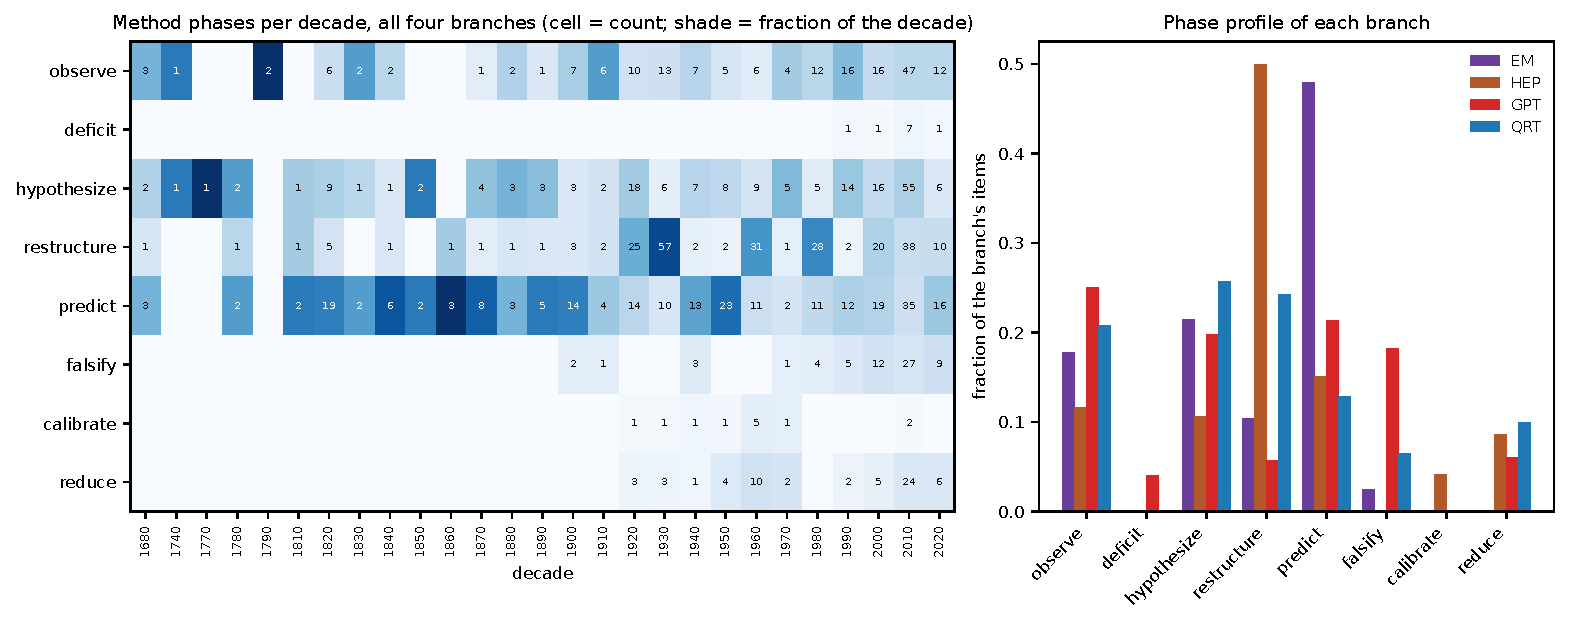
\includegraphics[width=\textwidth]{fig_evo_phases.pdf}
\caption{Left: events per decade by phase, all four branches (cell = count, shade = fraction of the decade). Right: phase profile of each branch.}\label{fig:evo_phases}
\end{figure}

\section{The philosophical structure, as graph operations}\label{sec:philosophy}
The phases are the operational form of positions in the philosophy of science. The correspondence below is stated with the data as evidence, and it records where the data do not support the received picture.
\begin{description}
\item[Falsification \citep{popper1959}.] A no-go or failed route. The reader's \EemFailedTotal{} failed derivations (R12) are falsifications of classical derivations by quantum observables, each resolved by a later route; in the nonclassicality network the first incident route of \EgptMnoGoFirst{} of \EgptMtotal{} model nodes is a pure no-go (\EgptMnoGoAny{} include one): a subtheory is introduced by what it cannot produce. In the history the anomaly steps (an observable with no model route, R2's precondition) are the falsifying events, and the data record their resolution as removal and replacement rather than as a route.
\item[Research programmes \citep{lakatos1970}.] A hard core that survives and a protective belt that is replaced. The data show the belt: all \EhepMfundAll{} fundamental model nodes, the \EhepMeffAll{} effective and the \EhepMcandAll{} candidate model of the history are removed, by absorption into successors and finally into the Lagrangian clusters; the \EhepMclusterAll{} cluster nodes and \EhepMframeKept{} of the \EhepMframeAll{} frames persist; the effect networks never remove their \EgptAxioms{} (GPT) and \EqrtAxioms{} (QRT) axiom nodes. The data do not show a protected core of \emph{model content} in the history: every model node that is not a frame or a cluster is replaced. What persists is structural (the frames that survive: unitary evolution, the observable postulate, the quantum field on Fock space; the particle Lagrangian is the one frame removed) and the end product (the clusters). The thesis records this as a finding about the data, not as a refutation of the reading, since absorption with a lineage edge (reduce) is different from refutation (falsify), and the engine distinguishes the two.
\item[Paradigm change \citep{kuhn1962}.] Restructuring of the state layer. In the graph a revolution is a sequence of ordinary operations (\cref{ch:limits}); on the year axis the restructure phase peaks in the \EdecadeMaxrestructure{}s with \EdecadeMaxrestructureN{} events, the re-partition of the one-particle Hilbert space into Fock space and sectors (R1/R3, back-edges). What the data do not show is incommensurability: the glue identifications across every restructuring (\EmergedGlue{} at 2026, growing through the 1920s--1930s) are concepts that keep their identity in the reader and the history while their layer and routes change.
\item[Holism \citep{duhem1954,quine1951}.] AND routes. \EemDeriveAND{} of \EemDeriveTotal{} derivations and \EemFailedAND{} of \EemFailedTotal{} failed routes of the reader have two or more inputs (model and state jointly); \EhepEntersAND{} of \EhepEntersTotal{} state$\to$model routes of the history are AND routes with occupation numbers. A failed AND route cannot by itself locate the faulty input, and the reader's resolutions (\cref{ch:readers}) are indeed new routes rather than deletions of one input.
\item[Explanation \citep{hempel1948}.] An M$\to$O route into an effect. The explanation lag of \cref{sec:arrivals} measures the years between an effect's appearance and its first model route: \EgptEffectsWithM{} of \EgptEffects{} effects have one, mean lag \EgptLagMean{} years, \EgptLagZero{} explained in their first year, Bell nonlocality after \EgptLagBell{} years. In the history every prediction is a single M$\to$O route (\EhepPredictsMO{} of \EhepPredictsTotal{}), the deductive-nomological form with the state dependence carried by the preceding \id{enters} routes.
\item[Discovery and justification \citep{reichenbach1938}; reduction \citep{nagel1961}.] The year of a route is its context of discovery (when its ingredients were in print), its status and polarity its justification; reduce routes (\id{lineage}, \id{subset}, \id{equiv}, \id{specializes}, \id{contains}; \Ephasereduce{} events) are the inter-theoretic reductions, and in the history they are the operations that make a model node removable: each of the \EhepRemovedModel{} removed model nodes (\EhepRemovedModelWithReduce{} of \EhepRemovedModel{}) is the source of a lineage or cluster-membership route (\EhepReduceRoutes{} such routes) naming its successor.
\end{description}

\section{The loop in time}
The eight phases, in the order of \cref{alg:step}, are observe $\to$ deficit $\to$ hypothesize $\to$ restructure $\to$ predict $\to$ falsify $\to$ calibrate $\to$ reduce. The evolutionary network shows the loop at three scales. At the scale of a decade all phases co-occur (\cref{tab:evo_merged_phases}). At the scale of a branch the profile is fixed by the signature. At the scale of a single node the order is visible as latencies: a witness and its effect appear together (observe), the effect's model route arrives \EgptLagMean{} years later on average (predict/explain), closures with the rest of the network follow with median latency \EGPTLatMedian{} years (TE2), and, in the history, a model node is reduced into its successor at a later step (TE5). The methodology written as an algorithm in \cref{ch:algorithm} is therefore also a description of the time series: \cref{alg:step} run once per event, with the solver's latency as the only quantity the engine does not compute.
